%!TEX root = ../these.tex

\section{Основные понятия}
\label{sec:cut.intro}

Проектирование управляющих программ
для технологического оборудования термической резки ---
это сложный, многоступенчатый процесс,
в котором можно выделить по крайней мере следующие этапы:
\begin{enumerate}
  \item
  Геометрическое моделирование и кодирование
  геометрии деталей / заготовок
  \item
  Разработка раскройной карты листового материала,
  \item
  Проектирование маршрута движения режущего инструмента
  по раскройной карте
  с учетом технологических ограничений оборудования
  \item
  Собственно генерирование управляющей программы
  для конкретного вида станка с ЧПУ
  \cite{bi:nc2020}
\end{enumerate}

Хотя вопросы, связанные с разработкой раскройной карты
\cite{bi:Nesting,bi:these.petunin}
(или говоря кратко --- \textit{раскроем}),
находятся вне темы данной диссертационной работы,
тем не менее,
невозможно не упомянуть
значительный вклад советских и российских исследователей
в теорию оптимизации раскроя.
Работы в этой предметной области
были начаты выдающимися учёными В.А.~Залгаллером
и Л.В.~Канторовичем
\cite{bi:Nesting0}
и продолжены в уфимской научной школе
Э.А.~Мухачевой и ее учениками:
А.Ф.~Валеевой,
М.А.~Верхотуровым,
В.М.~Картаком,
В.В.~Мартыновым,
А.С.~Филипповой, и др.,
см. например~\cite{bi:мухачева1984,bi:мухачева1998}.

В процессе раскроя порождается
графический файл,
содержащий информацию о геометрии
и расположении вырезаемых заготовок,
называемый
<<\textit{раскройная карта}>>.
Каждая деталь на листе
описывается при помощи внешнего замкнутого контура
и возможно одним или несколькими внутренними,
их расположение фиксировано в процессе раскроя
и служит входными данными для следующего этапа ---
маршрутизации режущего инструмента
(или коротко --- \textit{резки}).

Рассмотрим круг понятий, связанных с
\textit{маршрутом инструмента}
(маршрутом резки)
применительно к современным технологиям фигурной листовой резки~\cite{bi:book2020}.
В промышленном производстве единичного и мелкосерийного типа для
раскроя листовых материалов используются в основном такие технологии, как
лазерная, плазменная, газовая и гидроабразивная.
Целесообразность их
применения определяется разнообразными технологическими факторами,
включая свойства материала,
экономические требованиями к процессу резки,
технологические требованиями к качеству реза и пр.

Современные технологии резки предполагают как правило,
что для сохранения требуемой геометрии заготовки
траектория движения режущего инструмента не совпадает с
граничным контуром заготовки,
а проходит на некотором расстоянии от него
(по \textit{эквидистанте} контура,
см.~рис.~\ref{fig:toolpath}),
которое как правило составляет величину
равную половине ширины реза.
Это вызвано тем, что
часть материала вырезается
(<<сгорает>>, <<вымывается>> и т.п.)
в процессе резки.
Ширина же реза определяется
выбранной технологией резки,
толщиной и маркой материала,
заданной скоростью резки и
особенностями конкретного технологического оборудования,
используемого для резки.

\begin{figure}
  \centering
  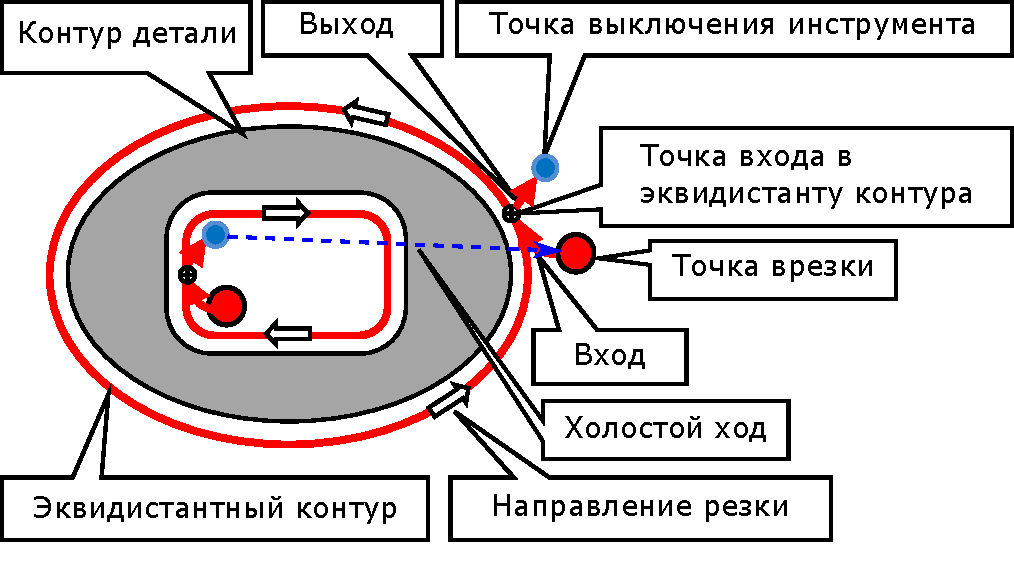
\includegraphics[width=0.8\textwidth]{toolpath.pdf}
  \caption{Элементы маршрута резки}
  \label{fig:toolpath}
\end{figure}

Следующая особенность листовой резки ---
необходимость предварительной \textit{врезки}
(пробивки) материала перед началом резки непосредственно по
эквидистантному контуру.
Пробивка материала сопровождается дополнительными деформациями материала,
поэтому производится на еще большем расстоянии от контура заготовки, чем
дистанция до эквидистантного контура
(за исключением случаев,
когда отверстия для точек врезки в листовом материале механическим способом готовятся,
например, просверливаются).
Иногда врезка может осуществляться непосредственно на границе материала
(<<врезка с края листа>>),
что позволяет значительно сократить
деформации материала и время на врезку.

Если используется
\textit{стандартная техника резки},
то каждый замкнутый контур вырезается целиком,
и  переход к следующей точке врезки происходит
с выключенным инструментом на \textit{холостом ходу}.
При этом точка выключения инструмента в общем
случае также не совпадает с точкой входа в эквидистантный контур,
по которому осуществлялась резка, и также, как и точка врезки, может
лежать вне эквидистантного контура.
Во многих случаях программирование точки выключения инструмента
допускается непосредственно на эквидистантном контуре.

Стратегия минимизации тепловых деформаций при термической резке
и требования к качеству реза порождают необходимость управления не
только выбором точек врезки,
но и  траекториями подхода к контуру
(lead-in)
и выхода из контура
(lead-out).
В зависимости от
конкретных условий
(вида термической резки, марки и толщины материала,
скорости резки, геометрической формы контура и пр.)
подход к контуру может осуществляться по дуге окружности,
касательная к которой совпадает с касательной к контуру в точке входа,
либо по прямой линии.
Аналогично,
после завершения резки выход из контура также может осуществляться с
включенным инструментом
либо по дуге, либо по прямой линии.
Необходимость этого может быть вызвана
тем, что в точке выключения инструмента может возникнуть <<вырыв>> или
оплавление части материала,
что приводит к искажению геометрии детали.
Уменьшение эффекта деформации заготовок
может достигаться специальными техниками резки,
например,
врезкой
в <<угловые>> точки заготовок.

На рис.~\ref{fig:toolpath}
на~стр.~\pageref{fig:toolpath}
представлены основные элементы маршрута резки:
\begin{itemize}
  \item Точка врезки
  \item Вход в контур (lead-in)
  \item Точка входа в эквидистанту контура
  \item Собственно траектория резки по эквидистанте контура детали
  \item Выход из контура (lead-out)
  \item Точка выключения инструмента
  \item Холостой путь до следующей точки врезки
  (как правило по прямой)
\end{itemize}

Проектирование маршрута резки заключается в выборе
этих элементов,
а также определении последовательности обработки контуров.
Задача поиска оптимальной
(в соответствии с некоторым критерием или группой критериев)
траектории перемещения режущего
инструмента является одной из наиболее
важных задач, возникающих при проектировании УП
в системах автоматизированного проектирования для
оборудования термической листовой резки
с~ЧПУ.

В настоящее время кроме \textit{стандартной техники резки}
<<по замкнутому контуру>>
(показанной на рис.~\ref{fig:toolpath})
при проектировании маршрута резки широко используются
так называемые
\textit{нестандартные техники резки}
(см.~рис.~\ref{fig:cut.non-std}).
Все техники фигурной резки на
машинах с ЧПУ можно разделить на 3 класса~\cite{bi:Petunin2015}:
\begin{enumerate}
  \item \textit{Резка по замкнутому контуру}
  (стандартная техника):
  сегмент резки содержит ровно один замкнутый эквидистантный контур
  заготовки, который вырезается целиком.
  \item \textit{Мультисегментная резка} контура:
  для вырезки одного
  контура используются не менее двух сегментов резки.
  \item \textit{Мультиконтурная резка}:
  резка предполагает вырезку нескольких контуров в одном сегменте.
\end{enumerate}

\begin{figure}
  \centering
  \subfloat[Резка с перемычкой]{
    \label{fig:cut.non-std.jumper}
    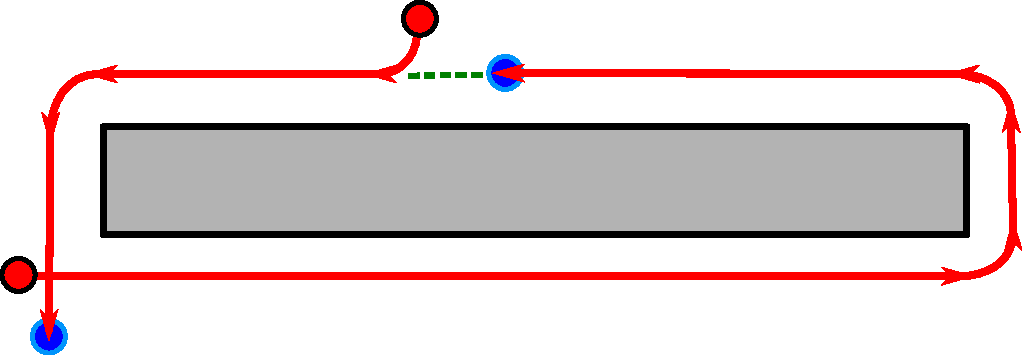
\includegraphics[width=0.6\textwidth]{jumper.pdf}
  }
  \\
  \subfloat[<<Восьмерка>>]{
    \label{fig:cut.non-std.8}
    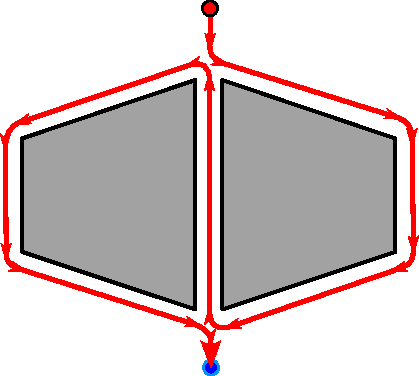
\includegraphics[width=0.3\textwidth]{8.pdf}
  }
  \subfloat[<<Змейка>>]{
    \label{fig:cut.non-std.snake}
    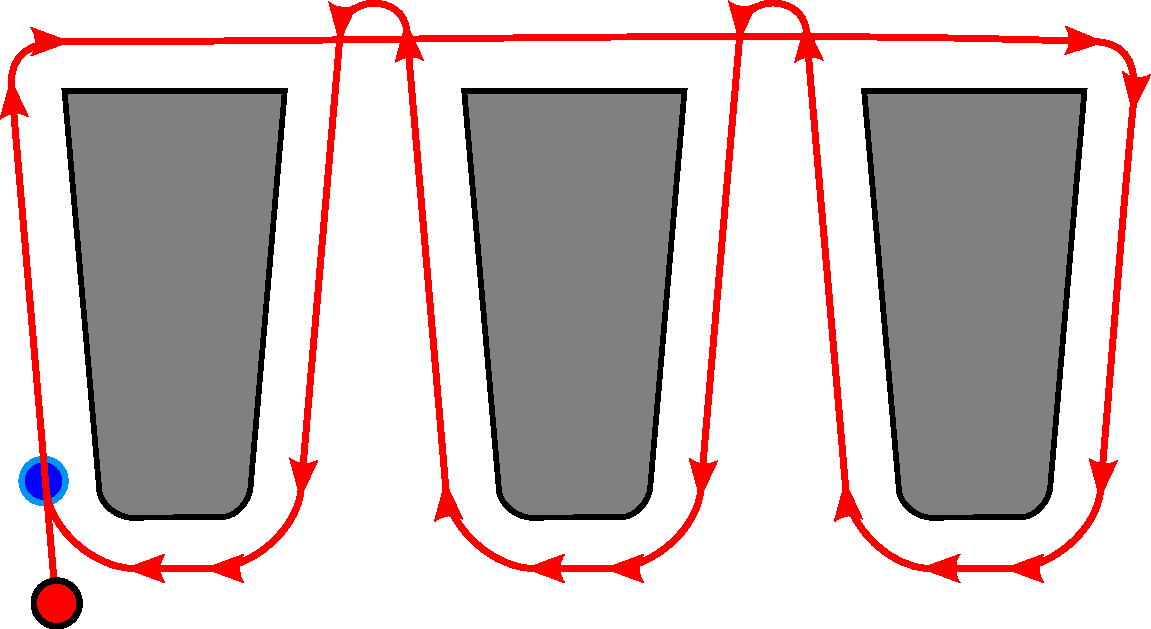
\includegraphics[width=0.5\textwidth]{snake.pdf}
  }
  \caption{Примеры нестандартных техник резки}
  \label{fig:cut.non-std}
\end{figure}

В качестве примеров
мультисегментной
резки можно привести
резку с перемычкой
(рис.~\ref{fig:cut.non-std.jumper}),
а мультиконтурной ---
«восьмерку»
(рис.~\ref{fig:cut.non-std.8}),
«змейку»
(рис.~\ref{fig:cut.non-std.snake}),
<<цепную резку>>, <<мост>>,
см.~\cite{bi:book2020}.
На практике используются и многие другие специальные техники резки,
но все их можно отнести к тому или иному из этих классов.
